\documentclass[11pt]{article}
\usepackage{acl2014}
\usepackage{times}
\usepackage{url}
\usepackage{latexsym}
\usepackage{graphicx}
\usepackage{dirtytalk}
\usepackage{caption}

\graphicspath{{images/}}
\captionsetup{justification=centering}

\title{An historical and political analysis of the panama papers.}

\author{Brou Boni Kevin \\
  {\tt kevin.brouboni@epfl.ch }\\
  Pavu\'e Cl\'ement\\
  {\tt clement.pavue@epfl.ch} \\
Roussaky Mohamed El Mehdi\\
{\tt mohamed.roussaky@epfl.ch} \\}

\begin{document}
\maketitle

\begin{abstract}
This project's idea was to understand why the Panama became a fiscal paradise and to try to determine the political and economic factors that make someone create an offshore entity. This way we will remember our conclusions about Panama Paper and avoid the same mistakes, hoping we will avoid similar in the future. Our conclusion is that several historical events directly impacted the number of entities in the country and the action of foreign governments to denounce the Panama as a fiscal paradise worked. However, we weren't able to have a clear analysis of the factor that incite people to create off-shore entities in the panama due to the intermediaries used in the process.

\end{abstract}

\section{Introduction}
The panama paper is the story of the leak of more than 11.5 million confidential documents detailing offshore companies used to hide money in the Panama, a fiscal paradise. All this document comes from the lawyer firm Mossack Fonseca, specialized in offshore financial service located in Panama. An anonymous person has sent the documents to the media in order to exploit them. In total 12 country presidents including 6 in activity, 128 political personality and 29 of the 500 richest persons in the world have been recognized guilty. Several athletes were also recognized guilty such as Lionel Messi or former French football legend Michel Platini. 

\section{Related work}

To help us do our project we take a look at work of the ICIJ on the panama papers. The way they represent the data as a graph really demonstrate how intermediaries and officers works. It was the most difficult part in the comprehension of the dataset and their work makes it easier for us. 

\section{Dataset Collection}
Beside the data provided by the ICIJ we used data from the heritage foundation of 2013. The mission of The Heritage Foundation 
\say{is to formulate and promote conservative public policies based on the principles of free enterprise, limited government, individual freedom, traditional American values, and a strong national defense.} according to their website. We used it as reference for economic and political analysis.

\section{Dataset description}
The data we downloaded on the ICIJ website was divided in five files. In total we have 213.634 off-shore companies registration from the 70's to 2015 with money coming from 159 different countries. 

Heritage's data is a brief sum up for each country of the situation of the human rights in the country, the economic situation in the country as for example the unemployment rate and finally the political situation of the country with for example the government spending. 

\section{Results and finding}
\subsection{Panama history through the data}

During the analysis phase of our project we created the following plot. It's describe the number of offshore company which has account in Panama.The number of offshore entities is sensitives to some historical events. We tried to understand which one. As we try to create a jurisprudence with the Panama let's try to understand why the number of entities may vary. To do so we will cut the previous graph to isolate the different phase and try to find the cause of this variation 
\begin{figure}[ht]
	\centering
    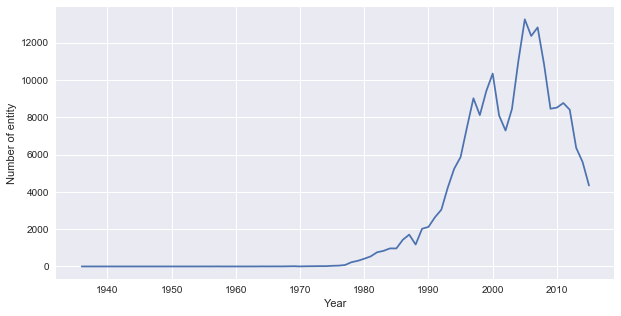
\includegraphics[width=7.7cm,height=4cm]{HistoricalContext}
    \caption{Evolution of the number of entities through the years}
    \label{fig:a}
\end{figure}

\subsubsection{1935 - 1960 Before the financial secrecy}
Back in this time Panama which economy relies on its mining activities and the Panama canal. As we can see below the number of offshore entities is almost zero. No abroad investments.

\begin{figure}[h]
	\centering
    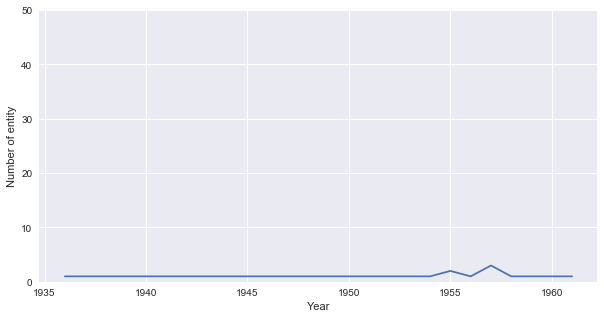
\includegraphics[width=7.7cm,height=4cm]{35-60}
    \caption{No offshore entities before the financial secrecy}
    \label{fig:b}
\end{figure}

\subsubsection{1960 - 2000 Before the financial secrecy}
In the 60's the Panamanian government has voted a law that enable corporate and individual financial secrecy. This is beginning of the panama as an fiscal paradise.

\begin{figure}[h]
	\centering
    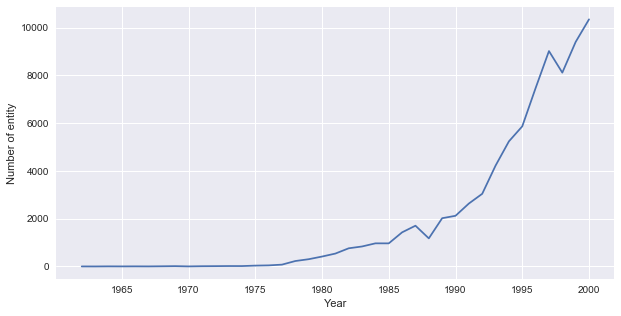
\includegraphics[width=7.7cm,height=4cm]{60-2000}
    \caption{The beginning of a fiscal paradise}
    \label{fig:c}
\end{figure}

We can clearly see the number of offshore entities rising. The law firm that will become Mossack Foseca is created in 1977, more or less when the curve start to rise. 
The two little decrease on the curve are due to the US interventions in Panama. 

\subsubsection{2000-2005 The OECD report effect on Panama}

In a report issued in 2000, the OECD identified a number of jurisdictions,including Panama, as tax havens according to criteria  it had established. Between 2000 and April 2002, 31 jurisdictions made formal commitments to implement the OECD’s standards of transparency and exchange of information. Panama was one of these 31 jurisdictions.

\begin{figure}[h]
	\centering
    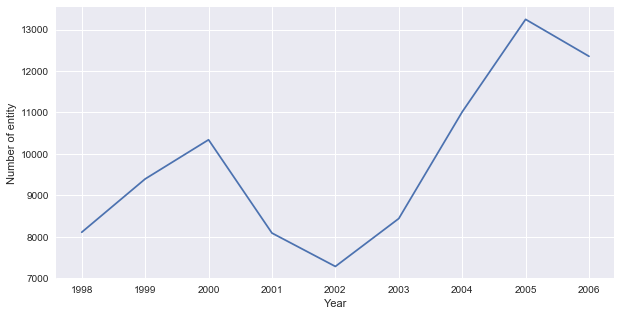
\includegraphics[width=7.7cm,height=4cm]{00-05}
    \caption{Decrease of the number on entities when the country was listed by OECD}
    \label{fig:d}
\end{figure}

As we can see the number of entities slightly decrease when the country was listed by OECD \cite{OECD_report}. People must have been scared of being revealed if they invest or continue their activities in Panama. 

\subsubsection{The sub prime crisis}
When we saw the fig1 we can see a decrease of the number of entities around 2009. This decrease happen during the sub prime crisis.

\begin{figure}[h]
	\centering
    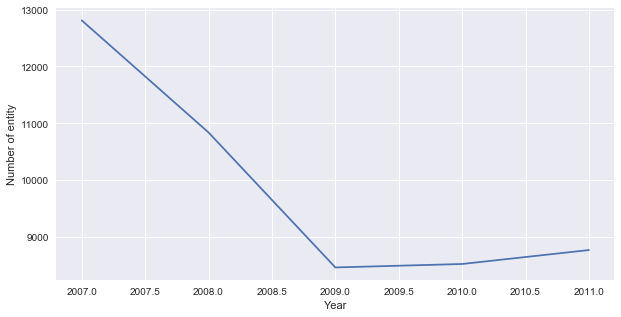
\includegraphics[width=7.7cm,height=4cm]{subprime}
    \caption{The effect of the subprime crisis}
    \label{fig:e}
\end{figure}

Our first thought when we try to find an idea for this project is that we will have an expansion of the number of entities at this period. It seems like it's the opposite. When we go deeper in the data we obtain this plot.

\begin{figure}[h]
	\centering
    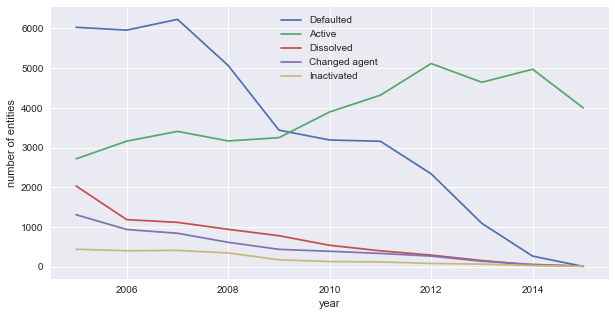
\includegraphics[width=7.7cm,height=4cm]{subprime2}
    \caption{The effect of the subprime crisis}
    \label{fig:f}
\end{figure}

Our first thought was right. The number of entities has decreased but the number of 'Active' account has increased and the number of 'Defaulted' which 'indicate that the company chose not to renew a payment or otherwise missed a payment necessary to remain active on the country's corporate registry. It does not necessarily mean the company defaulted.' according to the original website. Our assumption is that some people try to hide money from their governments and other took back their money, probably because they needed it to save their company.

\subsubsection{Conclusion}
As a conclusion for this first part, we saw that historical events can have a huge effect on the Mossack Fonseca activity. For example the action of the OECD benefit the rest of the world during the time the Panama was considered as a fiscal paradise, but they find a way to fake their willingness to stop financial secrecy due to the negative effect of being registered by the OECD. It's clear that the action of this organism is not vain.

\subsection{A political analysis of the world through the data}

During our analysis we did the following plot. 
\begin{figure}[h]
	\centering
    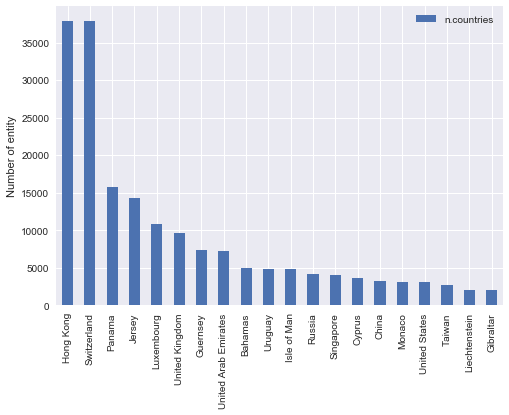
\includegraphics[width=7.7cm,height=4cm]{country}
    \caption{The top 20 most represented country in the dataset}
    \label{fig:i}
\end{figure}

Most of the entities come from an other fiscal paradise such as Honk Kong or Switzerland. There for when we try to obtain a result for a specific factor from the Heritage dataset we get something like this: 

\begin{figure}[h]
	\centering
    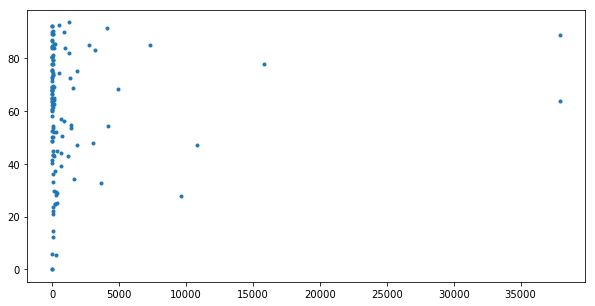
\includegraphics[width=7.7cm,height=4cm]{gov_spending}
    \caption{Impact of the government spending on the number of offshore entities}
    \label{fig:j}
\end{figure}    

Too many countries doesn't have enough entities to obtain a trustworthy result. Fiscal paradise like the Panama are used as an intermediaries for less transparency of the origin of the fund. Therefore we decided to create an heatmap resulting of the correlation of the numbers of entities in the dataset and the factors of Heritage. 

\begin{figure}[h]
	\centering
    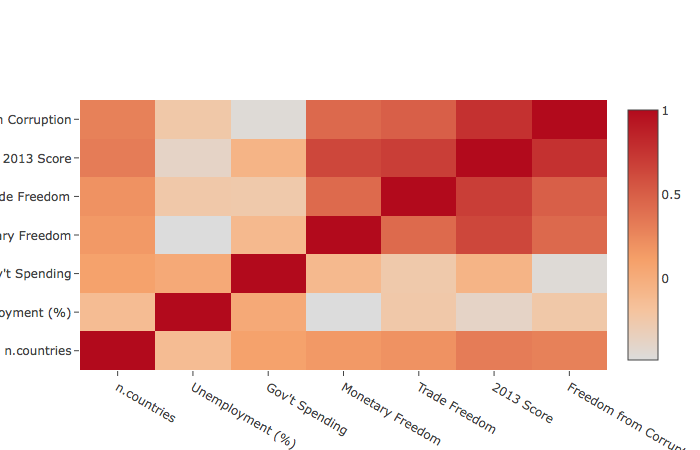
\includegraphics[width=7.7cm,height=4cm]{heat}
    \caption{Impact of the government spending on the number of offshore entities}
    \label{fig:j}
\end{figure}

The result we got was not we expected. At first we though that the financial situation of a country with factor like unemployment or the government spending will result the creation of offshore entities. But remember that most of the entities comes from fiscal paradise. So it's can be logical that the freedom from Corruption is one of the most important thing for someone who wants to hide something to their own government. Other factors seems to be important like trade and monetary freedom. These three factors are probably the representation of what a fiscal paradise is. It provide to investor financial secrecy.

To prove you that we would have need more data in order to determine these factors for non-fiscal paradise country, we will use a particular case, the one of Lionel Messi.He is accused by the Spanish government to have an offshore company named 'Mega Star Enterprises' in Panama\cite{Messi}. We actually found it and the found comes from Uruguay. So it's impossible to trace the money of someone coming from Argentina and working nowadays in Spain. 

An other trick used by Mossack Fonseca we would speak of the use of the name of the Red Cross to hide money. Indeed more than 80 accounts are registered with the name of the red cross. The lawyer firm though that account with this name won't be suspicious due to the reputation of the association. We provide in the reference an article of the NY post of possible consequences of this 'trick'. \cite{red_cross}

As conclusion for this part we found the factors that makes a fiscal paradise according to the data. We also learned that more data is needed in order to determine the factors for other countries. 

\subsection{Conclusion}

To conclude this project we achieve our first goal to have an historical analysis of the Panama, even if some events are perhaps not the only cause of a variation of the curve. Our second goal is partially achieved because we determine the factors of a fiscal paradise but not for a 'normal country'. One way to improve these analysis will be to used the other dataset on the ICIJ website and try to find matches between them. We also light up a dangerous trick used by Mossack Fonseca.

\bibliographystyle{plain}
\bibliography{sample}

\end{document}